%%Introduction

In this Section, we consider models with a photon, a W boson, a Z boson or a Higgs boson in the final state, 
accompanied by Dark Matter particles that either couple directly to the boson or are mediated by 
a new particle. The experimental signature is identified as \textit{V+MET}. 

These models are interesting both as extensions of models where the gluon provides 
the experimentally detectable signature, 
and as stand-alone models with final states that cannot be generated by the models in
Section~\ref{subsec:MonojetLikeModels}.

%%%Classification of models

%FIXME: CD - the tufte.cls on SVN does not like citep. Why? Will look into it later.
\begin{figure}[h!]
  \centering
    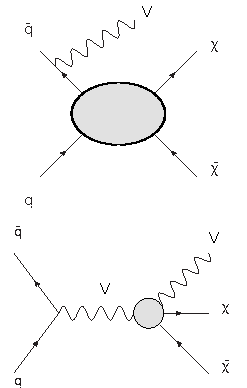
\includegraphics[width=0.5\textwidth]{figures/VPlusMET_EFT}
  \caption{Sketch of EFT models for V+MET searches, adapted from~\citep{Nelson:2013pqa}. \label{fig:VPlusMET_EFT}}
\end{figure}
% 
The models considered can be divided in four categories:
\begin{description}
 \item[EFT models where the boson is radiated from the initial state] As depicted in 
 the top diagram of Figure~\ref{fig:VPlusMET_EFT}, these  models follow the nomenclature and theory 
 for the EFT benchmarks commonly used by MET+X searches~\citep{Goodman:2010ku}. 
 \item[EFT models where the boson is directly coupled to DM] Shown in the bottom of Figure~\ref{fig:VPlusMET_EFT},
 these models allow for an EFT vertex that directly couples the boson to Dark Matter. 
 \item[Simplified models where the boson is radiated from the initial state] These models follow those
 already described in Section~\ref{subsec:MonojetLikeModels}, replacing the initial state gluon with a boson.
 \item[V-specific simplified models] These models postulate direct couplings of new mediators
 to bosons, e.g. they couple the Higgs boson to a new scalar~\citep{Carpenter:2013xra}. 
\end{description}

The following Sections describe the models within these categories, 
the parameters for each of the benchmark models chosen,
the studies towards the choices of the parameters to be scanned, 
and finally point to the location of their Matrix Element 
implementation. 

\paragraph{Simplified models with ISR boson radiation}

Searches in the jet+MET final state are generally more sensitive
with respect to final states including bosons, due to the much 
larger rates of signal events featuring quark or gluon radiation with 
respect to radiation of bosons~\citep{Zhou:2013fla}, 
in combination with the low branching ratios if leptons from 
boson decays are required in the final state. 
The rates for the Higgs boson radiation is too low for these models 
to be considered a viable benchmark~\citep{Carpenter:2013xra}.

However, the presence of photons~\citep{Khachatryan:2014rwa, Aad:2014vka}, 
leptons from W and Z decays~\citep{Khachatryan:2014tva, Aad:2014vka, ATLAS:2014wra} 
and W or Z bosons decaying hadronically~\citep{Aad:2013oja}
allows to reject the background more effectively, making Z/gamma/W+MET searches 
still worth comparing with searches in the jet+MET final state. 

% The three commonly chosen EFT benchmarks for Dirac dark matter that are 
% kinematically distinct for what concerns the observables used in 
% MET+X searches~\footnote{[CD: we would need a plot here, or a reference to 
% monojet section where this is shown]} and span a wide range of MET spectrum in 
% the boson+MET searches are, in the notation of ~\citep{Goodman:2010ku}, 
% the D1 (scalar SM/WIMP interaction), D5 (vector-vector interaction) and D9 
% (tensor interaction) operator. 

The case for searches with W bosons in the final state is strenghtened by the 
presence of particular choices of couplings between the WIMP and the up and 
down quarks which enhance W radiation~\citep{Bai:2012xg}, in the case of the exchange
of a vector mediator in the s-channel. 
We consider three sample cases for the product of 
up and down quark couplings to the mediator $\xi$:
\begin{itemize}
 \item No couplings between mediator and either up or down quarks~($\xi=0$);
 \item Same coupling between mediator and each of the quark types~ ($\xi=1$);
 \item Coupling of opposite sign between mediator and each of the quark types~($\xi=-1$);
\end{itemize}

The $\xi=-1$ case produces constructive interference between the two 
diagrams in which a W is produced from an initial state of an up and 
a down quark. This in turn increases the cross-section of the process 
and the hardness of the spectrum of missing transverse energy or 
transverse mass used for the searches. The sensitivity of the W+MET search for 
this benchmark in the case of constructive interference surpasses 
that of the jet+MET search. 

The above considerations lead to the choice of a vector mediator exchanged in the s-channel
as the main benchmark model, in the case of a W/Z boson or a photon are 
radiated in the initial state. 

\textbf{[CD: Plots I would like for this following section:
1. mT for Wlep, 2. MET for gamma, 3. MET for Z, 4. (wishful thinking) fat jet mass for Whad]}

The parameters for the definition and characterization of this model are: 
\begin{itemize}
 \item the mass of the DM particle ($m_{DM}$);
 \item the mediator mass ($m_{Med}$);
 \item the mediator width ($\Gamma_{Med}$);
 \item the couplings between the DM and the mediator ($g_{DM}$), 
 and between the mediator and the initial state quarks ($g_{SM}$);
 together with the product of the couplings between the mediator and up/down quarks ($\xi$);
 \item the chirality of the couplings between DM and mediator, 
 and between mediator and initial state quarks (vector-vector, axial-vector, axial-axial, vector-axial).
\end{itemize}

The DM and mediator mass ($\mathbf{m_{DM},m_{Med}}$) are scanned independently. 
Different kinematic distributions are obtained with a scan of 
\textbf{N} points in the DM/mediator mass plane, as shown in Figure~\ref{
insert here plots from Andy and Marie-Helene}. The spacing
of the points is chosen because \textbf{[CD: we need to justify this.]}

The couplings between the DM and the mediator $\mathbf{g_{DM}}$, and the couplings
between mediator and initial state quarks $\mathbf{g_{SM}}$ are scanned indipendently
following the recommendation for the jet+MET models
\textbf{[CD: link to monojet parameter scan]}. 
\textbf{[CD: do we have a plot of the dependence of the kinematics on the couplings?]}. 
The products of the couplings of the mediator to up and down quarks $\xi$ needs to be considered
for the three cases separately in the case of the W+MET signature. 
Figure~\ref{insert here figure by Kerstin Hoepfner} shows that
the constructive and destructive interference options have 
a similar kinematics. It is therefore recommended to generate 
two out of the three coupling ratio options ($\xi$=1 and $\xi$=0) and rescale 
the third. 
\textbf{[CD: Kerstin's plot of mT for different values of $\xi$ - 
how to make it more clear that we can rescale?
Or: can we show analytically that having two out of three is sufficient?]}. 

The \textbf{mediator width} is chosen to be the minimal possible width
for decays in quarks and Dark Matter assuming the couplings chosen
for the scan point, as in Equation~\ref{insert here monojet width eqn once Sarah is done and I can add label}. 
The width of this mediator as a function of the mediator mass 
\textbf{[CD: or some other plot, just to show it does not explode 
and that we are treating $\xi$ correctly]} is shown in Figure~\ref{insert here
figure of width for xi=0 and xi=1}. \textbf{[CD: is there any plot
of the dependence of the MET from the mediator width? This should be the same as the 
monojet, small difference in what happens to the ISR and MET, so we can just leave
the rescaling to larger widths to theorists and trust their width is not too large
so that they incur in PDF effects etc. Does this also hold for $M_{Wjet}$?]}

Similarly to the considerations made for the same model in the jet+MET case, 
the \textbf{chiral structure of the couplings}
does not change the kinematics of the main variables used for the 
search~\textbf{[CD: this will need a plot to be confirmed]}, 
so we recommend to restrict to one of the cases, e.g. the axial-vector coupling case for
SM and DM particles to the mediator respectively. 
\textbf{[CD: using axial-vector and justifying it with suppression at DD may not be
correct, see D'Eramo et al on RGE, will add paper link]}

These models are generated at leading order with MadGraph 2.2.2, and parameter
cards can be found on SVN \textbf{[CD: how to put this in write-up?]}.
The parton shower is done using Pythia 8, with a matching scale of... 
\textbf{[CD: need to figure this out.]}

\paragraph{EFT models with direct DM-boson couplings}

A complete list of effective operators with direct DM/boson couplings for
Dirac DM, up to dimension 7, can be found in~\citep{Cotta:2012nj}. 

Following the notation of~\citep{1212.3352}, the dimension 5 benchmark models 
from this category have a Lagrangian that includes terms such as:

\begin{eqnarray}
\frac{m_W^2}{\Lambda_5^3} ~\bar{\chi} \chi ~W^{+ \mu} W^{-}_\mu
+ \frac{m_Z^2}{2 \Lambda_5^3} ~ \bar{\chi} \chi ~ Z^\mu Z_\mu ~.
\end{eqnarray}
 
where $m_Z$ and $m_W$ are the masses of the $Z$ and $W$ boson, $W^{\mu}$ and $Z^{\mu}$
are the fields of the gauge bosons, $\chi$ denote the Dark Matter fields 
and $\Lambda_5$ is the effective field theory scale. This operator 
induces signatures with MET in conjunction with Z and W bosons at tree level,
while at loop level it induces couplings to photon pairs and $Z \gamma$ through W loops. 
\textbf{[CD: I believe the paper but I couldn't write this down. How much detail do we want here?]}. 







\paragraph{Specific simplified models}


%%%

%%This is left here in case we want to recommend EFT benchmarks?
% \begin{description}
%  \item[Vector interaction with vector-vector couplings (D5)]. For both jet+MET and boson+MET searches, the kinematic of this operator corresponds to that of couplings that are vector-axial (D7), axial-axial (D8) and axial-vector (D6). In the case of W boson radiation, the three coupling scenarios $\xi=1,0,-1$ should be investigated. This operator populates the high MET
%  \item[Tensor interaction (D9)]. As shown in Figure \textbf{[CD: add picture from Andy]}, this operator populates a higher MET range with respect to the other operators chosen. 
%  \item[Scalar interaction (D1)]. This operator has the lowest cross-section and sensitivity at colliders in this final state, as DM production from light quarks via a scalar interaction is suppressed with respect to heavy quarks. However, it has the hardest MET spectrum of the EFT operators chosen, and results obtained using this operator as benchmark may be used for recasting signals with a similarly hard MET distribution.~\footnote{Q for Andy/M-E: ZZchichi max gamma: is it the same kinematics regardless of DM? See fig. 2 of ATLAS monoZ.}
% \end{description}
